\chapter{Nanomaterial functionalisation modulates hard protein corona formation} \label{ProteinCorona}

%\epigraph{\textit{I Have divers times endeavoured to see and to know, what parts the Blood consists of; and at length I have observ’d, taking some Blood out of my own hand, that it consists of small round globuls driven thorough a Crystalline humidity or water: Yet, whether all Blood be such, I doubt.}}{Antoni Van Leeuwenhoek}

%\begin{center}
%    \textit{The contents of this chapter are under review with Nanoscale Horizons}
%\end{center}

The work in this chapter extends on the accurate modelling of graphene oxide nanomaterials to investigate changes in protein structure upon adsorption on the material. Using molecular dynamics simulations, we study the evolution of protein structure in response to interfacial interactions on the bio-nano interface. To understand the impact of structural changes over simulation times of hundreds of nanoseconds, we require a comprehensive analysis pipeline that investigates these changes from multiple perspectives. Here, we probe the varying adsorption behaviours of apolipoprotein c-III and the effect of functional groups in modulating protein aggregation on the nanomaterial. We use two functionalisations of graphitic materials --- graphene oxide and double-clickable graphene oxide.

\edit{Contributions for this work are as follows: \textbf{Mohamed Ali al-Badri} and \textbf{Christian D. Lorenz} conceived and planned the research. \textbf{Mohamed Ali al-Badri} performed the calculations. \textbf{Mohamed Ali al-Badri, Paul Smith} and \textbf{Christian D. Lorenz} analysed the data and \textbf{Mohamed Ali al-Badri} prepared the final manuscript.}
%Contributions for this work are as follows: \textbf{Mohamed Ali al-Badri}: Conceptualisation, Methodology, Software, Validation, Formal analysis, Investigation, Writing - original draft, Visualisation. \textbf{Paul Smith}: Methodology, Software \edit{development for analysis scripts}, Validation, Formal analysis, Visualisation.
\clearpage

The protein corona is an obstacle to exploiting the exotic properties of nanomaterials in clinical and biotechnology settings, with potential applications in DNA sequencing, point of care testing and drug delivery vehicles. The formation of the protein corona is driven by dynamic atomic scale interactions at the bio-nano interface, which are impenetrable using conventional experimental techniques. Here, we use molecular dynamics simulations to study the effect of graphene-oxide (GO) functionalisation on apolipoprotein-c3 (apo-c3) adsorption. We develop an analysis pipeline, encompassing binding energy calculations to protein structure analyses employing \edit{Uniform Manifold Approximation and Projection for Dimension Reduction (UMAP)} and machine learning clustering. We find that apo-c3 is denatured by adsorption on GO, largely driven by the large energetic contributions of electrostatic interactions such as $\pi$-$\pi$ stacking of aromatic amino acids to pristine graphene regions. The enthalpic contribution of such binding event outweighs the intraprotein bond enthalpy required to maintain the protein tertiary structure. Through denaturing and exposing buried hydrophobic residues, the protein backbone is stabilised by forming $\beta$-bridges, which serve as binding motifs for protein-protein interactions that drive further protein aggregation on the nanomaterial surface. When adsorbing on double-clickable azide- and alkyne-double functionalised graphene oxide (C2GO), apo-c3 largely retains its tertiary structure. Binding with the nanomaterial surface is dominated by weaker van der Waals interactions that are dispersed over the protein surface, where charged protein residues are sterically hindered by azide functional groups. The apo-c3 N-terminus is the binding motif for C2GO adsorption, leaving the  conformation of the C-terminus unchanged, hence conserving the lipid binding function of apo-c3.

\section{Introduction}

Graphene-oxide (GO) is a semi-ordered 2D material that shares many novel mechanical and electronic properties with graphene. It is utilised in applications including ion trapping, desalination, electronics, chemistry and biomedicine.\cite{yuan2017enhanced, zhu2010graphene, chung2013biomedical} GO is a promising platform for \textit{ex} and \textit{in vivo} biological applications --- such as bio-sensing and therapeutics. Its electrochemical properties makes GO an attractive contender for bio-sensing applications such as single nucleotide polymorphism detection in DNA,\cite{bonanni2012inherently} next generation nanopore DNA sequencing \cite{heerema2016graphene} and point of care (PoC) applications for early virus detection using covalently linked immobilised monoclonal antibodies.\cite{afsahi2018novel} Therapeutically, the large surface area to volume ratio of 2D materials results in a large loading capacity for targeting molecules, fluorescent dyes and drug molecules for intravenous administration as well as photothermal therapy for cancer treatment.\cite{robinson2011ultrasmall, liu2013graphene, sun2008nano, zhang2010functional}  \\

Unfortunately the transition from \textit{in vitro} to clinical settings is held back by a chemically driven adsorption of serum proteins --- referred to as a protein corona --- upon their introduction to a biological medium.\cite{casals2010time, ke2017decade} A hard corona (HC) is a tightly bound monolayer of proteins at the nanoparticle interface. Subsequent protein layers adherent to the HC are referred to as the soft corona (SC).\cite{rocker2009quantitative} The character and composition of the HC define the nanomaterial's biological identity and therefore its biological fate, circulation time, cellular uptake and cytotoxicity.\cite{nierenberg2018formation, mei2018protein} HC formation has revealed highly variant protein composition profiles, sensitive not only to inter-species biological media \cite{solorio2017comparison} but also disease-specific influences in human GO coronas.\cite{hajipour2015personalized} Patient-specific or `personalised' protein corona profiles have since been utilised as a diagnostic tool for high-throughput, inexpensive and highly accurate early cancer detection.\cite{papi2019converting} \\

Modulating the HC character to overcome the disadvantages of 2D materials in biological applications through nano-functionalisation remains challenging.\cite{rampado2020recent} Extrapolating the sensitivity of nano-functionalisation to the aforementioned highly variant identity of the corona from experimental studies is incomplete and requires a better understanding of GO-HC interfacial behaviour to atomistic precision. Such an understanding is paramount to designing the next generation of biosensors and nanomedicines.\\

Azide- and alkyne-double functionalised graphene oxide (C2GO) has previously been proposed as a cancer targeting nanovector,\cite{mei2015synthesis} where click reactions conjugate targeting moieties on azide and trimethylsilyl (TMS)-alkyne functional groups.\cite{rubio2015solvent} In vitro, both C2GO and GO show varying HC character when exposed to serum proteins, which subsequently impacts their biological identities.\cite{mei2018protein} An experimental quality-by-design screening platform was used to unpick the HC character and evaluate its relationship with biological fate, cellular uptake and cytotoxicity. Using this, proteins that reduced material dependent toxicities were identified to play a role in diminishing cytotoxicity, including apolipoprotein C-III (apo-c3).\cite{mei2018protein} \\

Protein coronas are known to temporally evolve, leaving the total amount of protein constant but varying their composition according to binding affinity, known as the Vroman effect.\cite{vroman1980interaction} Upon the introduction of a nanomaterial to a biological medium, highly abundant proteins such as albumin, immunoglobulin G and fibrinogen bind to the nanoparticle surface in the early stages of the Vroman effect, followed by their replacement with high binding affinity proteins such as apolipoproteins and coagulation factors in the late stages of the Vroman effect.\cite{foroozandeh2015merging, ehrenberg2009influence, harnisch2000adsorption, goppert2005polysorbate, vroman1980interaction} The Vroman effect has previously been observed in computational and experimental studies of peptide, cellulose and fatty-acid binding on GO.\cite{radic2013competitive} \\

 Previously, MD has been used to study the interactions of GO with peptides to understand conformational transitions of amyloid-beta during adsorption,\cite{baweja_effect_2015} the hydration pattern of an adsorbed toy-model alpha-helix \cite{baweja2013hydration} and verification of enzyme active-site deformation following adsorption. \cite{sun_mechanism_2014} To the best of our knowledge, no MD simulations have so far studied protein adsorption on accurate models of GO, and have instead randomly placed oxidised functional groups on the GO surface. Accurate modelling of GO should reflect the semi-ordered structure of GO; composed of inhomogeneous regions of oxidised and unoxidised domains, where amorphous alcohol and epoxy groups make up the oxidised regions.\cite{sinclair2019modelling} \textit{Ab initio} MD simulations of GO show that semi-ordered models of GO are the most stable structures in vacuum as well as in liquid water.\cite{mouhat2020structure} Furthermore, we have recently shown the importance of accurate functionalisation and accounting for steric strain and edge functional groups in large scale MD simulations of GO, using generalised and bespoke electronic structure MD forcefield design.\cite{al2020accurate} In this work, we use molecular dynamics (MD) simulations to study protein denaturing through adsorption on GO and C2GO, to understand HC conformation-activity relationships through binding free energy, contact map, protein structure and solvent exposure analyses. We apply machine learning dimensionality reduction techniques to decode the spatio-temporal MD data that is hard to interpret into distinct protein secondary structure conformations.
%--------------------------------------
%
%               RESULTS
%
%--------------------------------------
\section{Results}
%
\subsection{Binding on the bio-nano interface}
%
In both GO and C2GO systems, apo-c3 readily adsorbs to the substrate and reaches a stable conformation over the course of the adsorption trajectory. To investigate the binding of apo-c3 to the GO and C2GO interface, we compute contact maps and free energies of binding that underpin the changes in protein structure following adsorption. These analyses probe interfacial dynamics that may play a large role in the formation of a protein corona around a nanomaterial upon its introduction to a biological medium. To identify adsorption of apo-c3 to the graphitic sheets we calculated the minimum distance over time between any heavy (non-hydrogen) atom of the protein to any heavy atom of the sheet (Fig.~\ref{fig:mid-dist-to-grap}). We also compute the minimum distance of each residue to the graphitic sheets over time. These are combined to produce a heatmap of contact probability between apo-c3 and GO/C2GO (Fig.~\ref{fig:contacts}B). The binding free energy is calculated according to the molecular mechanics with Poisson–Boltzmann and surface area solvation (MM-PBSA) method, implemented using g\_mmpbsa.\cite{kumari2014g_mmpbsa}\\

\begin{figure*}
    \centering
    \includegraphics[width=\textwidth]{figures/contacts-energies-fixed.png}
    \caption{MM-PBSA binding energy contributions per apo-c3 amino acid residue for GO and C2GO sheets, colour coded by magnitude (A), heat map showing contact probability of apo-c3 amino acid type with GO and C2GO functional group atoms (B) and adsorbed apo-c3 structure on GO and C2GO, protein amino acids at the graphitic interface are coloured by MM-PBSA binding energy contribution and hydrogen atoms have been omitted for clarity (C).}
    \label{fig:contacts}
\end{figure*}
%
The average binding free energy components for the GO-apo-c3 and C2GO-apo-c3 systems are given in Table 1. The binding free energy components are decomposed to per-residue contributions (Fig.~\ref{fig:contacts}A). In this way we can acquire a better understanding of each amino-acid's contribution to the binding free energy of the protein-nanomaterial complex. Per-residue binding free energy contributions are colour-coded by their interaction strength (blue to red) in the protein structure of the final configuration (Fig.~\ref{fig:contacts}C) for GO and C2GO, where each largely contributing amino acid residue has been illustrated and labelled explicitly. \edit{Note that the entropic contribution to the binding free energy is not calculated using high-throughput methods such as g\_mmpbsa, due to their computational cost. Therefore, the binding free energies in (Table 1) are computed to evaluate the relative binding free energy instead of the absolute free energy.}\\

The binding of apo-c3 to the graphitic substrate is driven by amino acids with the highest binding affinities from the beginning of the adsorption process. Apo-c3 residues 60-70 initiate binding with GO (Fig.~\ref{fig:mid-dist-to-grap}), most likely due to the high binding affinity of TRP65 to $\pi$-$\pi$ stack with pristine graphene domains on the GO surface, as well as GLU63 binding with positively charged (tertiary alkyl, phenol and carboxylic acid) carbon atoms (Fig.\ref{fig:contacts}A). From 100 ns apo-c3 binding to GO is driven by positively charged (HIS18, LYS21) and polar (THR20) residues (Fig.\ref{fig:contacts}A) interacting with oxygen containing surface functional groups. Accordingly, the binding free energy of GO-apo-c3 has a higher net contribution of electrostatic interactions when compared with C2GO-apo-c3, contributing -208 kJ/mol to the total binding free energy (Table 1). \\

In contrast, binding to C2GO is driven by both of the extreme N- and C-terminal ends of apo-c3, which also have the highest binding affinity to the C2GO substrate according to the MM-PBSA binding free energy analysis. The N-terminus serves as the main binding domain with C2GO, driven by negatively charged (GLU4, ASP5) and polar (SER10, GLN13) residues interacting with a TMS group and positively charged (tertiary alkyl, phenol and carboxylic acid) surface and edge carbon atoms (Fig.~\ref{fig:prot-c2go-contacts}). Meanwhile, charged amino acid residues contribute a net positive change in binding free energy of apo-c3 to C2GO  (Fig.~\ref{fig:contacts}A), stabilising C2GO-apo-c3 binding and a conserved apo-c3 tertiary structure. Charged amino acids are the only residues in apo-c3 that sterically hinder neighbouring amino acids from binding to the C2GO interface, and this is wholly achieved through azide functional groups, with the exception of ARG40 which is sterically hindered by a silanol group. However, the role of azide groups is not exclusively restricted to an agent for steric hindrance of amino acid side chains to the graphitic surface, as they drive the binding of hydrophobic amino acids in the extreme C-terminal end of apo-c3 (Fig.~\ref{fig:contacts}A,B). Unlike GO-apo-c3, C2GO-apo-c3 binding is dominated by van der Waals interactions, contributing $-463.2$ kJ/mol to the total binding free energy (Table 1). \\

\begin{table*}
\caption{Binding energy components from MM-PBSA calculations performed on the MD trajectories of adsorbed apo-c3 on GO and C2GO sheets. Stronger binding components have been highlighted in bold.} \label{table:pbsa}
\resizebox{\textwidth}{!}{\begin{tabular}{SSSSSS}                         \toprule
     {} & {\vdw (kJ/mol)} & {\elec (kJ/mol)} & {\polar (kJ/mol)} & {\apolar (kJ/mol)} & {\binding (kJ/mol)}\\ \midrule
    {GO}      &{-338.8±0.8}&{\textbf{-208.3±1.5}}&{\textbf{422.2±5.5}}&{-31.9±0.1}&{-156.8±5.3} \\ \midrule
    {C2GO}    &{\textbf{-463.2±0.9}}&{-135.7±1.0}&{420.5±3.0}&{\textbf{-47.5±0.1}}&{\textbf{-225.9±2.8}} \\ 
    \bottomrule
\end{tabular}}
\end{table*}
In the case of GO-adsorbed apo-c3 binding is dominated by electrostatic interactions (Table 1) with a locus around two binding hotspots --- LYS21, TRP65 (Fig.~\ref{fig:contacts}A) ---  which stabilises unfolding of the protein. This is due to the enthalpic contribution of this binding outweighing the bond enthalpy of the intraprotein interactions maintaining the tertiary structure. Due to the changes to the apo-c3 native state tertiary structures induced by adsorption, apo-c3 has a significantly higher conformational entropy. The energetic stabilisation of a denatured protein is attributed to the conformational entropy of amino acid side chains, which would be a barrier to recovering the native state tertiary structure.\cite{leach1998exploring} In contrast, the enthalpic contribution in C2GO-adsorbed apo-c3 is more dispersed over the surface (Fig.~\ref{fig:contacts}A) and is on average dominated by weaker (van der Waals) interactions (Table 1), thus the intraprotein interactions maintaining the tertiary structure are not compromised by any energetic spikes caused by strong binding in any location on the complex interface.
\subsection{Protein structure}
Changes to protein structure during adsorption --- leading to protein denaturing or deformation --- are evaluated using secondary structure, intramolecular hydrogen bonding and solvent-accessible surface area (SASA) analyses. Protein native contacts indicate changes in secondary structure due to adsorption, their temporal evolution is calculated using the define secondary structure of proteins (DSSP) algorithm\cite{Kabsch-1983} and protein intra-molecular hydrogen bonds. 
%
\subsubsection{DSSP and hydrogen bonds}
%
To understand the dynamic progression of denaturing in GO-adsorbed apo-c3, DSSP and hydrogen bond analyses indicate the sequential loss of secondary structure and number of intra-molecular hydrogen bonds respectively. The number of protein intramolecular hydrogen bonds over time (Fig.~\ref{fig:dssp}B) complement the DSSP results (Fig.~\ref{fig:dssp}A) at a higher resolution and are invariant to the DSSP algorithm criteria for defining strands, helices or coils. It shows that over time, unlike C2GO-adsorbed apo-c3, GO-adsorbed apo-c3 has a dynamic character, sporadically gaining or losing hydrogen bonds. These high spatio-temporal hydrogen bond frequencies stabilise intrachain contacts by recovering the loss of hydrogen bonds, indicating structural reorganisation is taking place during adsorption. \\

Loss of secondary structure in C2GO-adsorbed apo-c3 is transient, with temporary loss of $\alpha$-helix character spanning residues 30-40 (Fig.~\ref{fig:dssp}A). In contrast, GO-adsorbed apo-c3 $\alpha$-helix character is lost irreversibly \edit{for residues 30-35 and 55-60} (Fig.~\ref{fig:dssp}B), concomitantly with the formation of $\beta$-turns whose lifetime range from tens to hundreds of ns and persist throughout adsorption \edit{(Fig.~\ref{fig:dssp}C)}. A decrease of $\alpha$-helices accompanied by an increase of $\beta$-strands elsewhere in the protein is a characteristic observed in experimental secondary-structure analysis of denatured protein libraries using vacuum-ultraviolet circular dichroism.\cite{matsuo2007secondary} Within the initial 150 ns of adsorption, $\alpha$-helices spanning residues 1-10, 30-33 and 40-50 transition to coils (Fig.~\ref{fig:dssp}A). Subsequently at 200 ns, the C-terminus loses it's $\alpha$-helix character in residues 55-65, the lost hydrogen bonds (Fig.~\ref{fig:dssp}B) are recovered through forming $\beta$-turn motifs (Fig.~\ref{fig:dssp}A) and stabilising the apo-c3 protein backbone (Fig.~\ref{fig:dssp}C) for the remainder of adsorption until 400 ns. $\beta$-turns remain stable in a solvated state, potentially serving as recognition motifs of protein-protein interaction,\cite{tyndall2005over} until binding takes place with other proteins. Both L4-S7 and W54-T56 transitioned from an alpha-helix to type-I and type-II $\beta$-turns, respectively, whereas S48-K51 transitioned from a coil to a type II $\beta$-turn. 
\begin{figure*}
    \centering
    \includegraphics[width=\textwidth]{figures/dssp-hbonds-fixed.png}
    \caption{Define Secondary Structure of Proteins (DSSP) algorithm applied to the MD trajectory of apo-c3 adsorption with GO and C2GO (A), the number of intramolecular hydrogen bonds per amino acid residue throughout adsorption (B) and illustration of $\beta$-turns induced in GO-adsorbed apo-c3 following denaturing (residues \edit{L}4-S7, S48-K51 and W54-\edit{V57}), pink and grey structures respectively correspond to the initial and final adsorption conformations (C).}
    \label{fig:dssp}
\end{figure*}
%--------------------------------------
%              CLUSTERING 
%--------------------------------------
\subsection{Clustering}
UMAP dimensionality reduction is a useful approach to map high dimensional data of MD protein backbone coordinates trajectories to a lower dimensional protein configuration space.\cite{mcinnes2018umap-software} This is due to the better performance of UMAP in preserving local and global structure relationships compared with conventional dimensionality reduction techniques such as principle component analysis (PCA) or t-distributed stochastic neighbour embedding (t-SNE). A projection of the high dimensional spatio-temporal MD data into a low-dimensional space is used to identify distinct protein structures, bridging pathways and global relationships between distinct configurations. It is also a practical tool for visualising what is otherwise a vast dataset. \\

The number of clusters in the protein configuration space reflects the number of ensembles the protein backbone adopts, namely the distinct structures of apo-c3 during the entire adsorption process. Using this and the visualisation of protein structures corresponding to each cluster, we can see that apo-c3 has higher structural variance when adsorbing on GO than on C2GO, which have 13 and 10 clusters, respectively (Fig.~\ref{fig:umap}). GO-adsorbed apo-c3 clusters show how the protein sequentially undergoes a process of reorganisation (Fig.~\ref{fig:umap}) driven by interchain hydrogen bonding interactions (Fig.~\ref{fig:dssp}B) due to the binding interactions with the GO surface (Fig.~\ref{fig:contacts}A). \\

The temporal evolution of apo-c3 adsorption follows the cluster numbers in the protein configuration space (Fig.~\ref{fig:umap}). The pathways between clusters are synonymous with the DSSP analysis, corresponding to transitions between configuration states where apo-c3 secondary structure either gains or loses $\alpha$-helix, $\beta$-bridge or coil character. In both cases of GO and C2GO adsorption, the reorganisation process requires transitions to discrete intermediary states (clusters) before converging to a stable complex (Fig.~\ref{fig:umap}). The stable complex may or may not recover its secondary structure following these transitions, corresponding to whether it has or has not been denatured via the adsorption process. This is indeed the case in GO-adsorbed apo-c3, which has undergone drastic structural changes and retains some of its N-terminus (Fig.~\ref{fig:umap}) but loses the C-terminus secondary structure. In contrast C2GO-adsorbed apo-c3 does recover most of its secondary structure, where different cluster pathways transition between the highly conserved native backbone (Fig.~\ref{fig:umap}), which is indicative of binding deformations instead of protein denaturing. Note that the images of the protein backbone annotating the clusters only approximate secondary structure character and are not as accurate as the state-of-the-art characterisation of the secondary structure using DSSP analysis (Fig.~\ref{fig:dssp}). 

\begin{figure*}
    \centering
    \includegraphics[width=\textwidth]{clustering_both.pdf}
    \caption{Uniform Manifold Approximation and Projection (UMAP) dimensionality reduction of protein backbone denaturing during adsorption on GO (top) and C2GO (bottom) nanosheets. Separate clusters show clear separation of distinct protein backbone secondary structures. Protein structures corresponding to each cluster are coloured by secondary structure (helices in blue, loops in pink) on top of an overlay of all cluster conformations (grey).}
    \label{fig:umap}
\end{figure*}

\subsection{Solvent exposure}
As a result of structural changes induced by adsorption, the hydration of the apo-c3 amino acids change and contribute to potential protein aggregation \textit{in vivo}. As the structure of apo-c3 changes during adsorption on GO, solvent exposure is increased significantly over multiple regions of the amino acid sequence (Fig.~\ref{fig:sasa}A). Some residues will have a larger solvent-accessible surface area (SASA) after adsorption due to change in conformation. Some residues will have a smaller SASA after adsorption either due to a change in conformation leading to new protein-protein contacts or due to interaction of the residue with the nanomaterial in question. There is a correlation with increased solvent exposure in regions where apo-c3 forms $\beta$-turns, as analysed by DSSP and illustrated in (Fig.~\ref{fig:dssp}). The $\beta$-turns remain in this solvated state, potentially serving as recognition motifs for protein-protein interactions until binding to other proteins \textit{in vivo} or \textit{in vitro}.\cite{tyndall2005over} As well as increased solvent exposure of the GO-adsorbed apo-c3 C-terminal helix (residues 47-65), the EVRPTSAVAA minimotif (residues 70-79) has a consistently higher solvent exposure than the native state of apo-c3 in solution (Fig.~\ref{fig:sasa}A,B). These exposed hydrophobic residues keep the adsorbed complex in a disordered state until it can coalesce with its protein/lipid environment. In contrast, the solvent exposure of apo-c3 adsorbed to C2GO is limited to isolated short sequences leaving the conformation of most of the C-terminal helix region (residues 47-65) unchanged (Fig.~\ref{fig:sasa}A).

\begin{figure*}
    \centering
    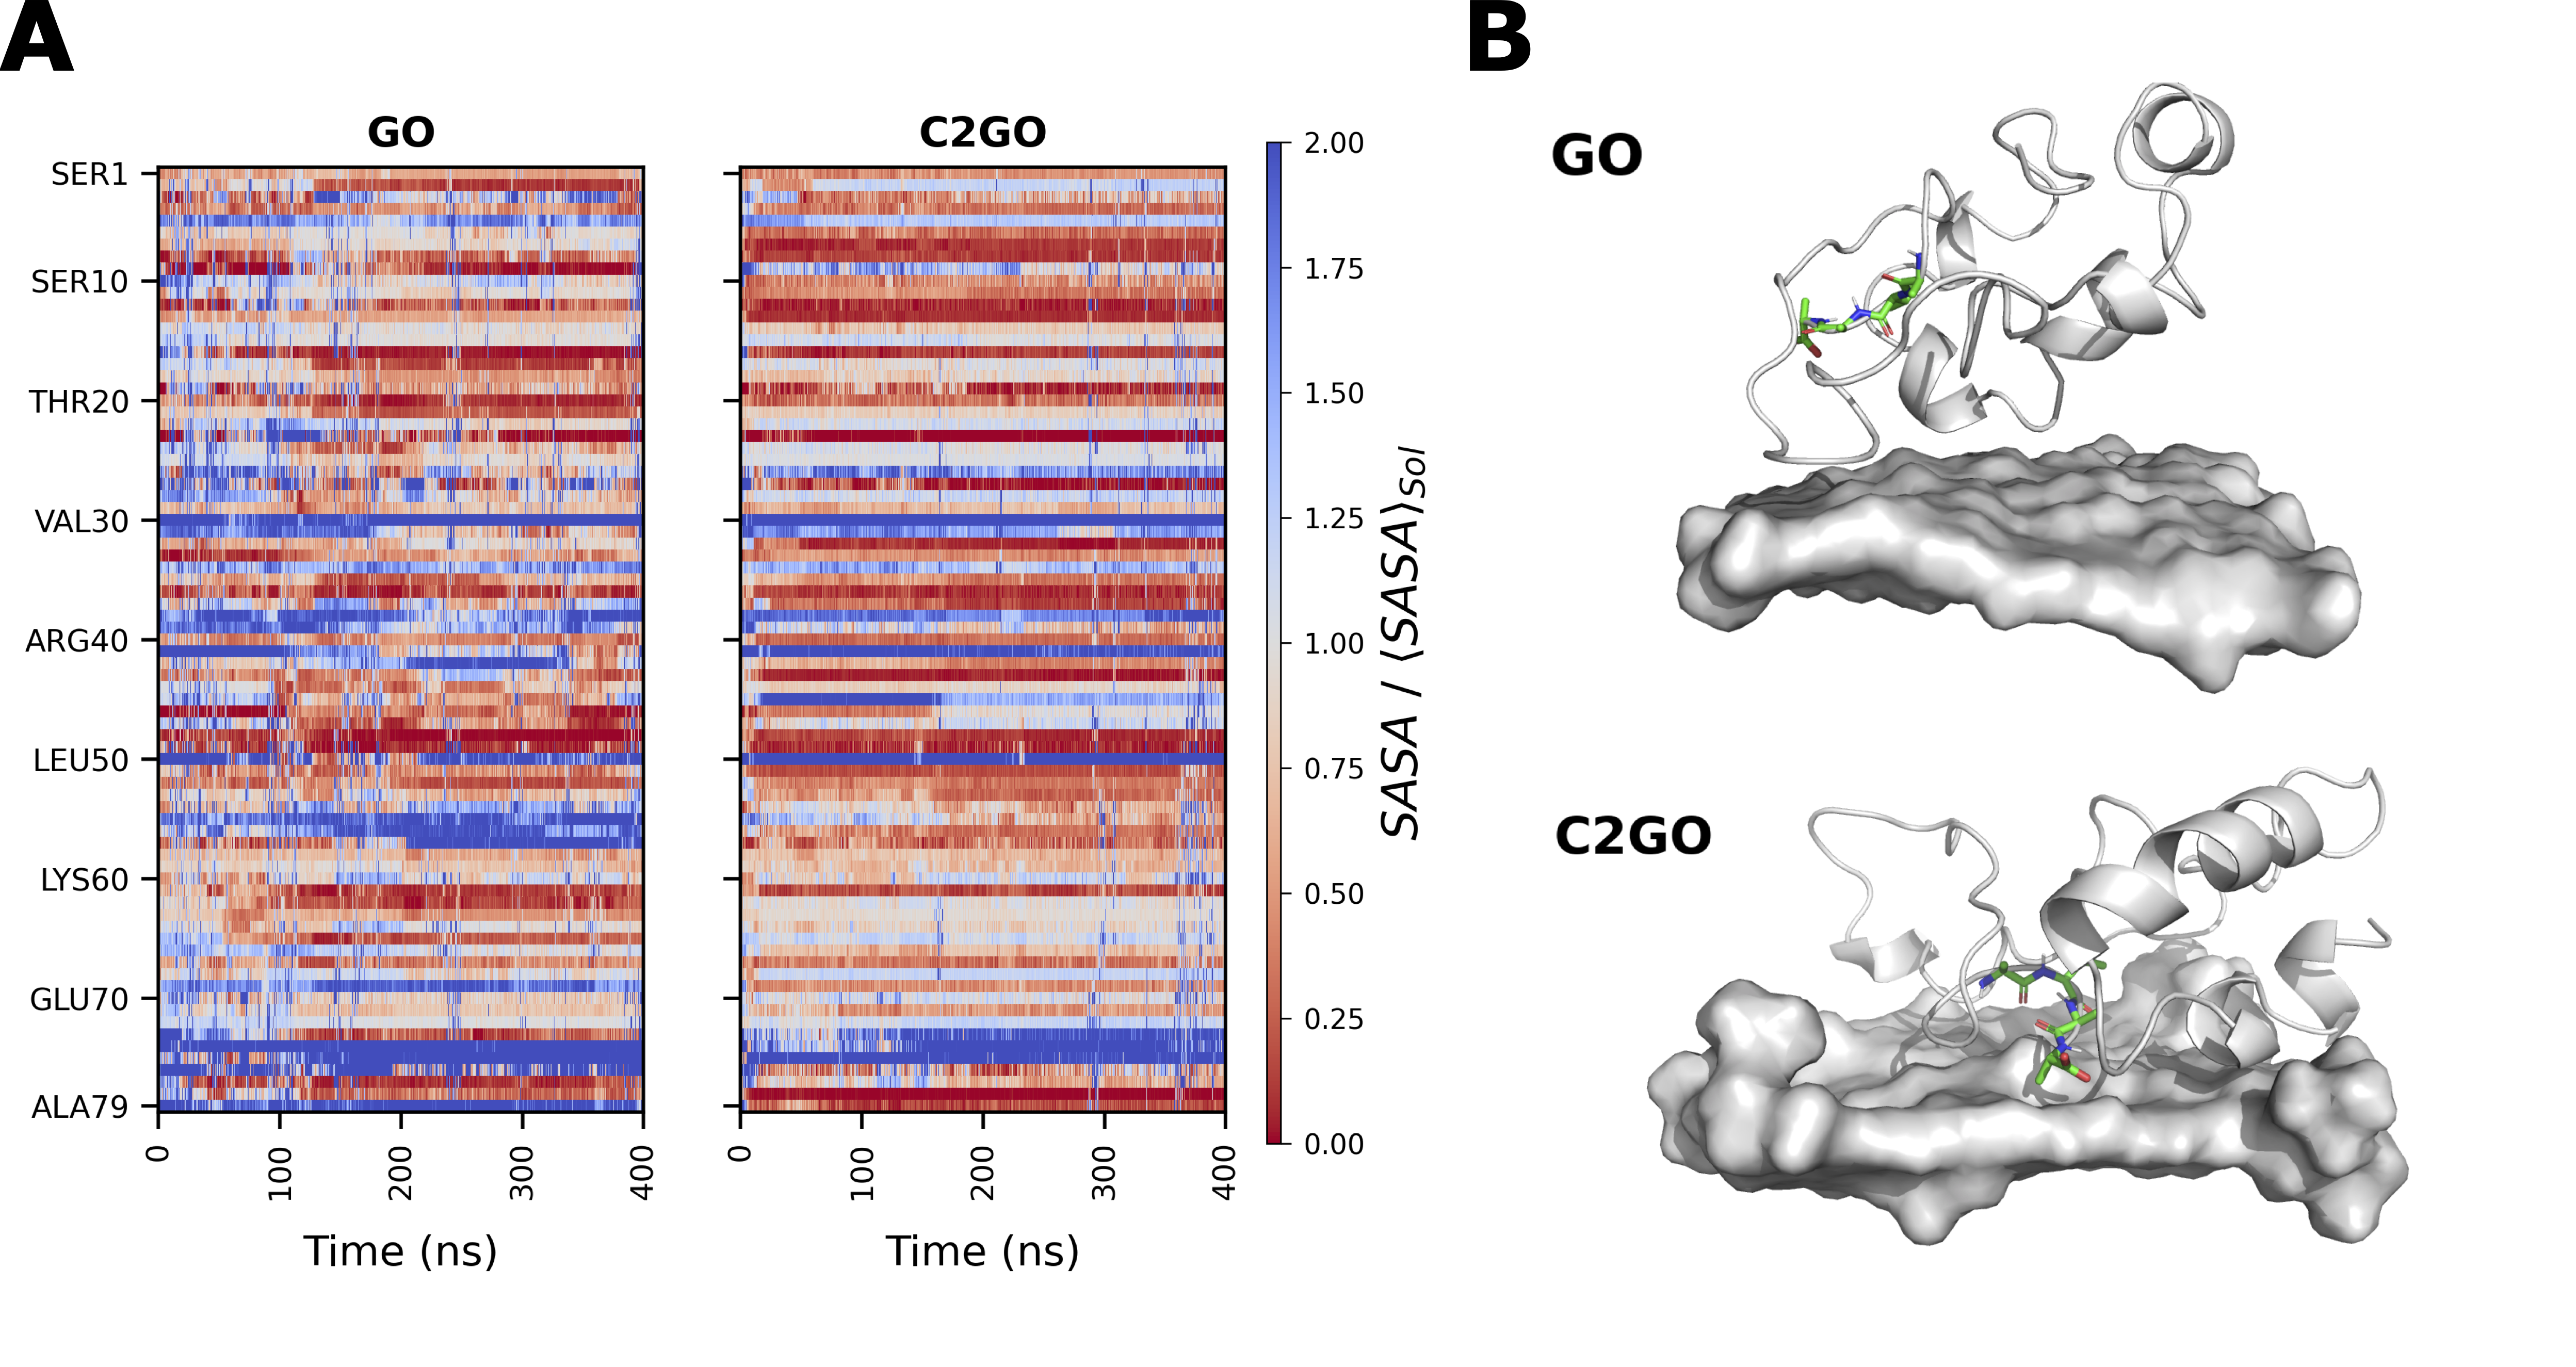
\includegraphics[width=\textwidth]{sasa-snapshot.png}
    \caption{The surface accessible surface area (SASA) of apo-c3 amino acid residues during adsorption to GO and C2GO sheets, normalised by average SASA of apo-c3 in solution (A) and illustration of exposure of the AVAA minimotif in the C-terminal region of apo-c3 to solvent in GO adsorption and contrasting structure in C2GO adsorption, the nanomaterials are represented as a surface for clarity (B).}
    \label{fig:sasa}
\end{figure*}

Previous work has found that the C-terminal region of apo-c3 is essential for mediating lipid binding, with the N-terminal region (residues 1-40) playing a limited secondary role.\cite{sparrow1977lipid, meyers2017aromatic, lambert1996effect} Solvent exposure analysis of the C-terminal helix expresses the conservation of its lipid-binding function from a physio-chemical perspective. These results may in part delineate the experimentally observed preferential uptake of corona-coated C2GO to corona-coated GO by J774 cells.\cite{mei2018protein} 
%--------------------------------------
%               METHODS 
%--------------------------------------
\section{Methods}
\subsection{Nanomaterial structure}
%
We have modified a Python package \cite{make-graphitics-github} to generate azide and trimethylsilyl (TMS)-alkyne functional group conjugated rectangular graphene-oxide flakes.\cite{albadri2020accurate-github} The package improves on the commonly applied protocol, of randomly placing oxidised functional groups, which we now know is an incomplete model of graphene-oxide structure.\cite{al2020accurate, mouhat2020structure} Instead, we recreate the two-phase nature of oxidised and unoxidised graphene domains observed in microscopy experiments \cite{Pacile2011, Cai2008, Saxena2010, Erickson2010} in accordance with our recent study of accurate large scale modelling of graphene oxide.\cite{al2020accurate}
\subsection{Molecular Dynamics}
%
MD simulations were performed in GROMACS version 2020.1 on the ARCHER2 AMD EPYC Zen2 (Rome) 64 core CPUs at 2.2 GHz or Nvidia V100 GPUs. The all-atom OPLS forcefield was used to simulate the classical simulations. A position restraint algorithm was applied to all non-solvent atoms during equilibration. The $\sim$130\,\AA\, cubic simulation box was fully solvated with TIP3P water molecules. The system net charge was neutralised by adding four sodium ions into the system. The system was relaxed energetically using steepest-descent energy minimisation for 50000 steps with an energetic step size of 0.01 kJ/mol. The minimisation was terminated after the maximum energetic contribution was lower than a threshold of 1000.0 kJ/mol/nm. NVT and NPT equilibration was performed for 100 ps using two separate modified velocity-rescaling thermostat --- with a stochastic term to ensure generating the canonical ensemble --- coupling temperature to velocities for graphene and solvent molecules (NVT),\cite{bussi2007canonical} where a temperature of 300K was maintained and 1 bar using the Parrinello-Rahman barostat (NPT). The Verlet cut-off scheme was employed to generate pair lists and the electrostatic interactions were calculated using the Particle-Mesh Ewald algorithm. Both electrostatic and van der Waals interactions were cut off beyond 1.2 nm. All bonds involving hydrogen atoms were constrained using the LINCS algorithm. Production simulations were run for 400 ns using a timestep of 1~fs. Analysis was performed using the MDAnalysis package \cite{mda, oliver_beckstein-proc-scipy-2016, Michaud-Agrawal-2011} and its analysis modules.\cite{araya2014characterization,smith2019interaction} To identify hydrogen bonds we used the hydrogen bond analysis tool \cite{smith2019interaction} implemented
in MDAnalysis. We used the MDTraj \cite{McGibbon2015MDTraj} implementation of DSSP. 

\subsection{Contact maps}
Contact maps between apo-c3 and the graphitic sheets were calculated using a hard cutoff of \SI{5.0}{\angstrom} between any two heavy (non-hydrogen) atoms. Data over the final \SI{50}{\nano\second} were used for the contact maps, as during this period apo-c3 was stably adsorbed to both GO and C2GO. We constructed contact maps between between GO/C2GO and each specific residue of apo-c3 (Fig.~\ref{fig:prot-go-contacts} and \ref{fig:prot-c2go-contacts}), as well as contact maps between GO/C2GO and each amino acid regardless of its position in the sequence (Fig.~\ref{fig:contacts}B).
%
\subsection{PBSA binding energies}
We post process the last \SI{10}{\nano\second} of MD trajectories using molecular mechanics with Poisson–Boltzmann and surface area solvation (MM-PBSA) analysis implemented using g\_mmpbsa,\cite{kumari2014g_mmpbsa} to obtain a relative order of binding of apo-c3 to the different graphitic nanosheets. The energetic components of the binding free energy are the changes in the system potential energy \textit{in vacuo}, the polar and non-polar solvation energies. The potential energy accounts for bonded (bond, angle and torsion) and non-bonded (van der Waals and electrostatic) energetic terms. Polar solvation energy is the electrostatic contribution to the solvation free energy and is estimated using the Poisson-Boltzmann equation. The non-electrostatic contribution to the solvation free energy accounts for forces between solute and solvent, which are calculated using the solvent accessible surface area (SASA).\cite{kumari2014g_mmpbsa} 
%
\subsection{UMAP dimensionality reduction}
We used the atomic coordinates of apo-c3 to obtain an ensemble of distinct structural conformations when adsorbed to the graphitic sheets. We first centre and align the structures along their backbone atoms, using every tenth frame (\SI{50}{\pico\second}) from the trajectory. We then use the uniform manifold approximation and projection for dimension reduction (UMAP\cite{mcinnes2018umap-software}) algorithm to embed the atomic coordinates of heavy atoms of apo-c3 into a two-dimensional space. UMAP constructs a graph of the points in the high-dimensional space, then optimises a low-dimensional representation of the graph such that the topological distance is preserved to a degree in the embedding.\cite{mcinnes2018umap-software} Therefore, similar conformations that are close in the high-dimensional space will also be close in the reduced space. We set the \code{n\_neighbours} and \code{min\_dist} hyperparameters to 15 and 0.0, respectively, with the latter being a requirement if the points in the reduced space are to be clustered. We use HDBSCAN\cite{mcinnes2017hdbscan}, implemented in scikit-learn\cite{scikit-learn}, to cluster the apo-c3 conformations in the embedded space. We identify representative structures of each conformation by calculating the mean structure of a conformation, then finding the structure with the smallest RSMD from this mean structure.
%
\subsection{SASA solvent exposure}
To quantify the solvent exposure of amino acids during adsorption, we calculated the solvent accessible surface area of each residue of apo-c3 over time. To understand how the conformational changes lead to exposure of residues that are buried in the native state, we normalised the SASA time-series by the mean SASA of each residue of the protein in solution. We used the final \SI{50}{\nano\second} of apo-c3 solution for determining the mean SASA of each residue. Values greater than and less than \num{1} indicate, respectively, increased and decreased exposure to the solvent (Fig.~\ref{fig:sasa}A). The SASA was calculated using the ``rolling-ball" Shake-Rupley algorithm,\cite{SHRAKE1973} implemented in MDTraj.\cite{McGibbon2015MDTraj} This approximates the SASA by effectively rolling a ball over each atom of the protein to define a surface, then examining how much of the each atom's surface is exposed to solvent as opposed to overlapping with surfaces of neighbouring atoms. The radius of the probe in typically set to \SI{1.4}{\angstrom} --- approximately the radius of a water molecule.


%--------------------------------------
%             CONCLUSIONS 
%--------------------------------------
\section{Conclusions}

 This work has dissected the protein structural changes induced by interactions of functional groups and protein residues on the bio-nano interface. Through adsorption on GO, apo-c3 shows denaturing of the secondary structure over large swathes of the protein sequence. Whereas C2GO-adsorbed apo-c3 has limited deformation, with most variance displayed in the N-terminus. The C-terminus of apo-c3 has previously been found to be responsible for lipid binding, with the N-terminus playing a limited secondary role.\cite{sparrow1977lipid, meyers2017aromatic, lambert1996effect} These findings correlate with experimental evidence of the increased cellular uptake of C2GO, as compared to GO, hard protein corona.\cite{mei2018protein} \\

Apo-c3 is found to denature upon adsorption to GO, according to solvent exposure, DSSP and conformational clustering analyses. Following adsorption on GO, apo-c3 forms 3 separate $\beta$-turns that serve as binding motifs for protein-protein interactions. These can aid in subsequent aggregation of serum proteins to the corona, contributing to the corona identity in vivo, hence complicating the targetability of the nanomaterial-corona complex. \\

The functional groups at the binding interface between the nanomaterials and apo-c3 set off a series of dynamic events that result in large-scale secondary structure changes. Contact distances, heatmaps and binding free energy calculations collectively describe the driving forces of the changes in protein structure following adsorption. The introduction of azide and TMS functional groups was sufficient to stop the denaturing of apo-c3 and the formation of $\beta$-turns that serve as protein-protein interaction binding motifs. We find that contact with azide functional groups correlate strongly with contact to other surface functional groups and therefore work cooperatively to maximise the binding surface at the bio-nano interface. Consequently, the C2GO-adsorbed protein is stabilised and is not pushed to structural deformation as is the case in GO-adsorbed protein. The results from this analysis pipeline suggest the causes of protein aggregation and cellular uptake are mediated by the aforementioned changes in protein structure. \\

This work indicates that the dynamic and functional role of adsorbed proteins may be a more important probe to understanding the protein corona, rather than quantifying a static image of its constituent proteins. MD simulations are a valuable tool for such an investigation and our analysis pipeline serves as a transferable method for understanding the structure/function relationship of dynamic protein-nanomaterial adsorption.

%Analysis methods are outlined in the SI, including contact maps (Supp. Note 1), MM-PBSA binding energy calculations\cite{kumari2014g_mmpbsa} (Supp. Note 2), UMAP dimensionality reduction\cite{mcinnes2017hdbscan, scikit-learn} and HDBSCAN clustering\cite{mcinnes2017hdbscan} (Supp. Note 3) and SASA solvent exposure\cite{SHRAKE1973, McGibbon2015MDTraj} (Supp. Note 4).
%\section*{Supplementary figures}
%
\begin{figure}[ht!]
    \centering
    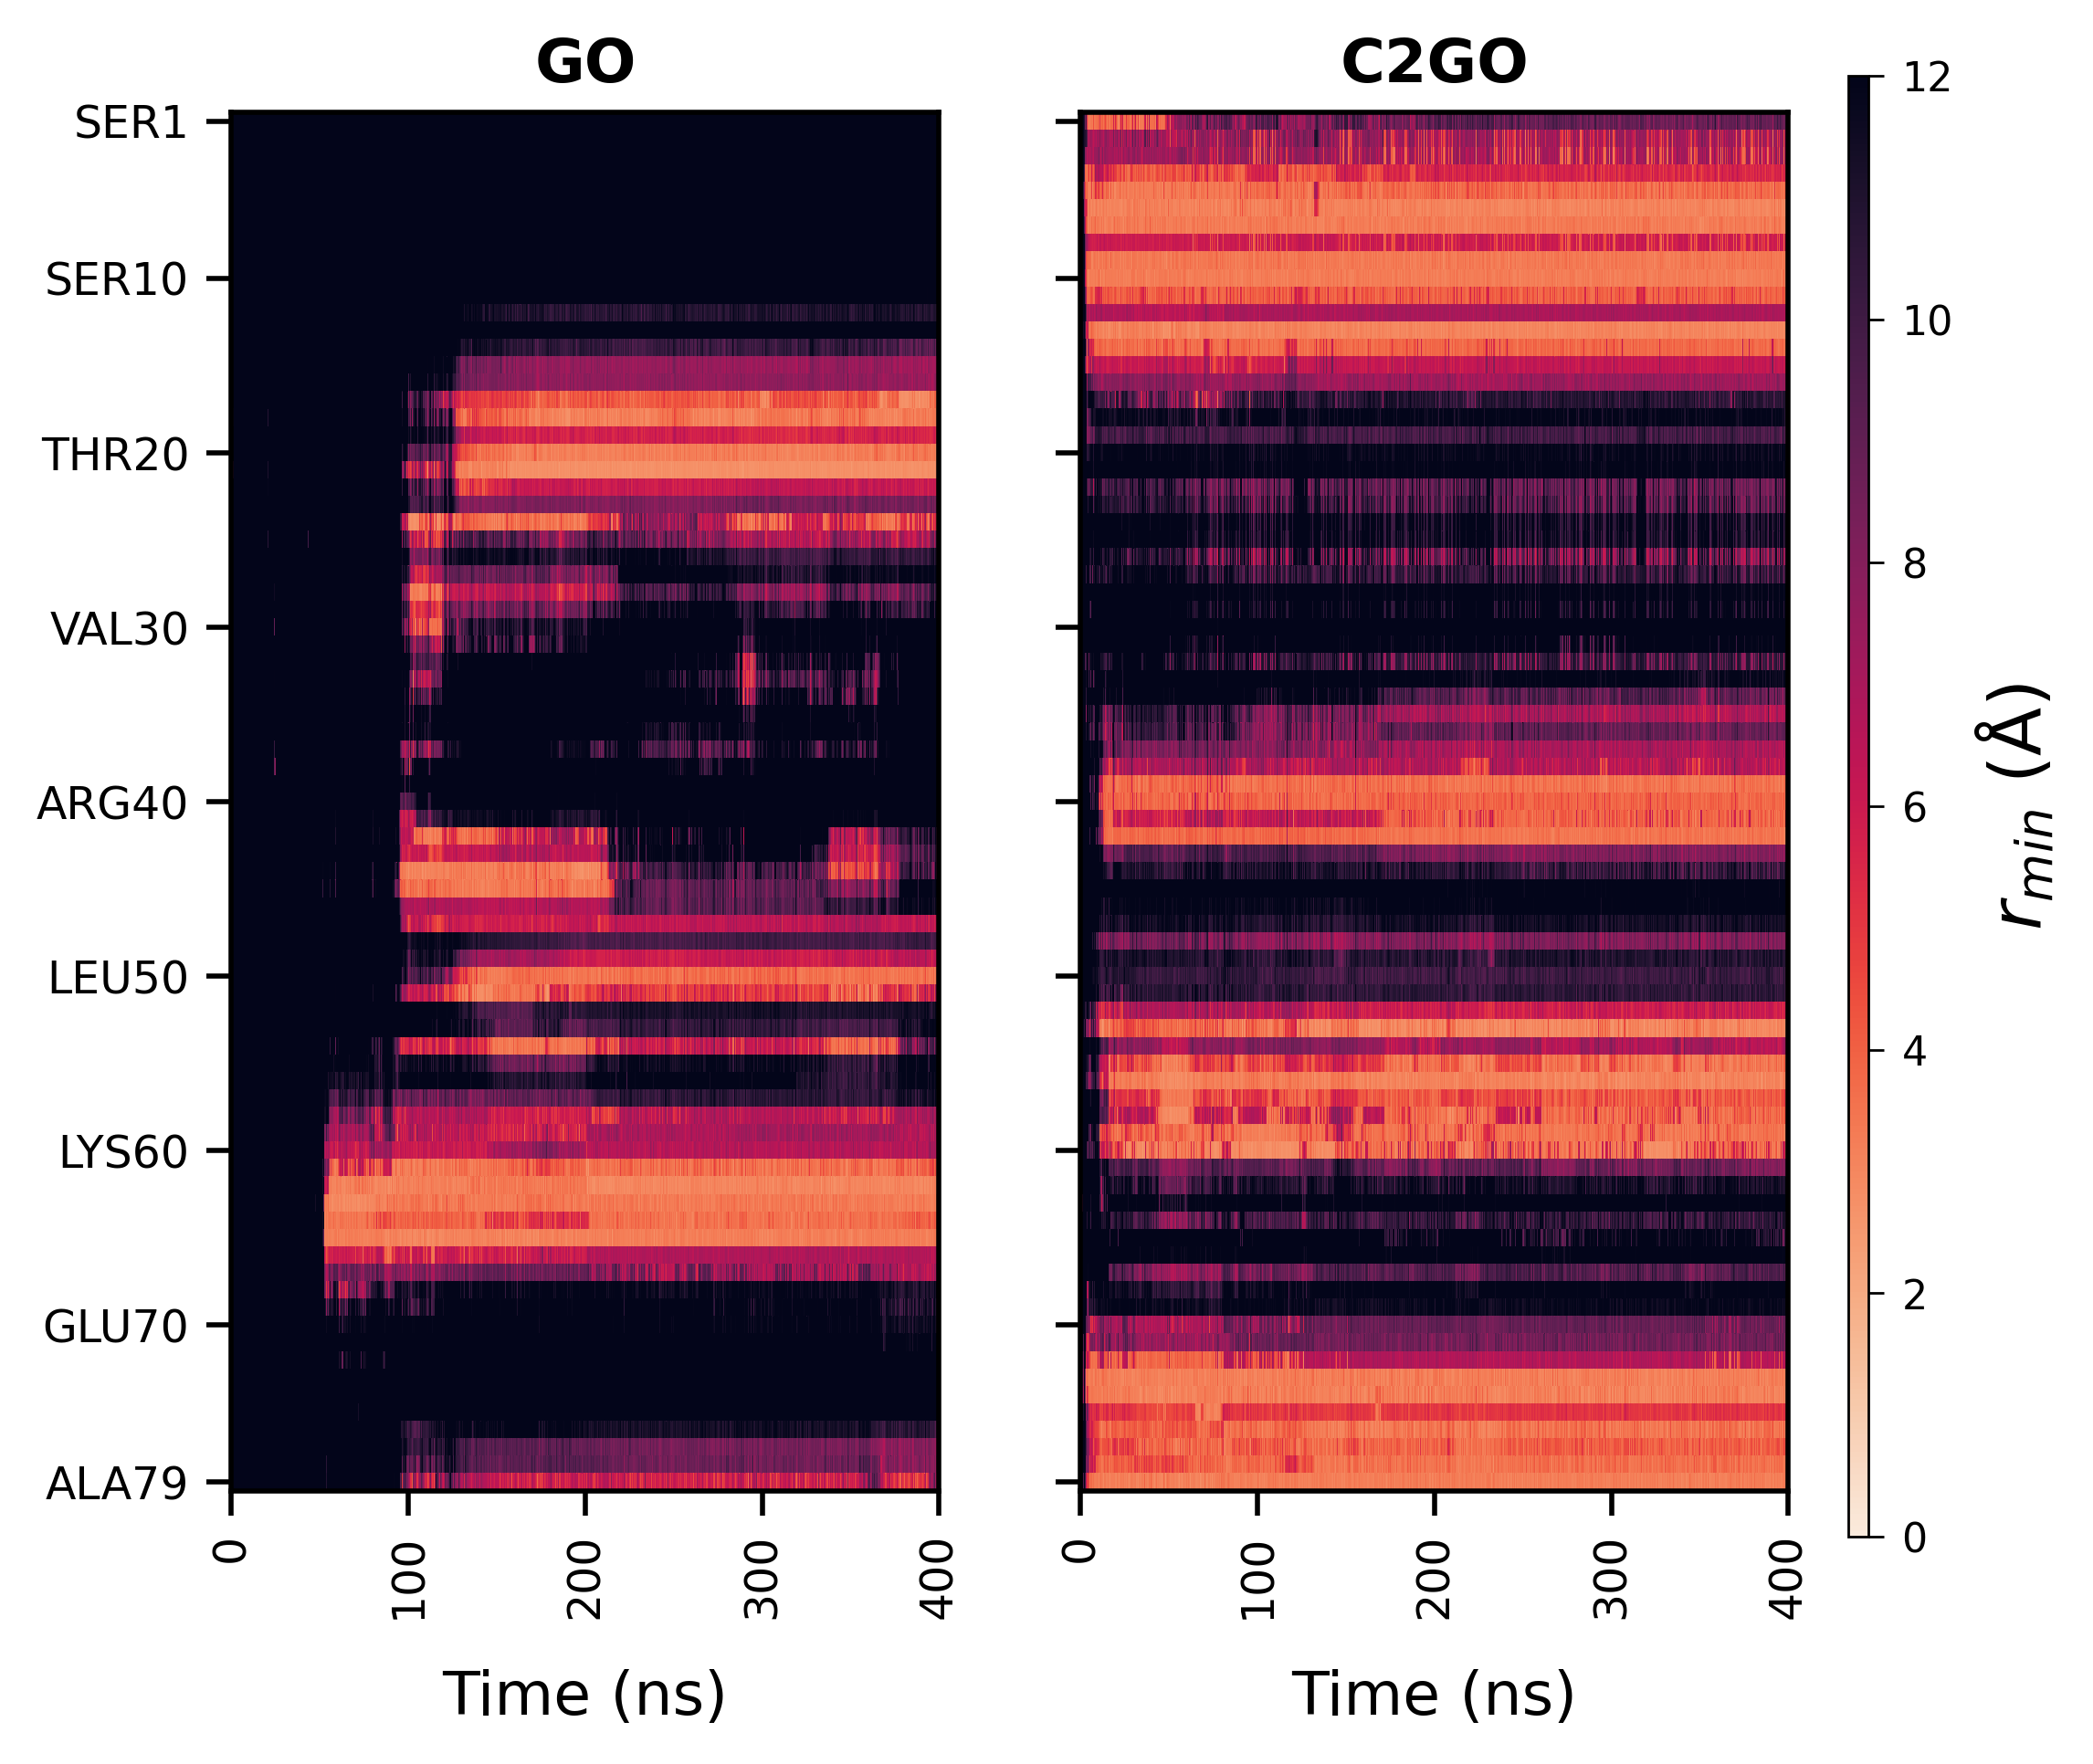
\includegraphics[width=0.8\linewidth]{SI_min-dist-to-grap.png}
    \caption{Minimum distance to any GO/C2GO heavy atom for each residue in apo-C3.}
    \label{fig:mid-dist-to-grap}
\end{figure}

\begin{figure}
    \centering
    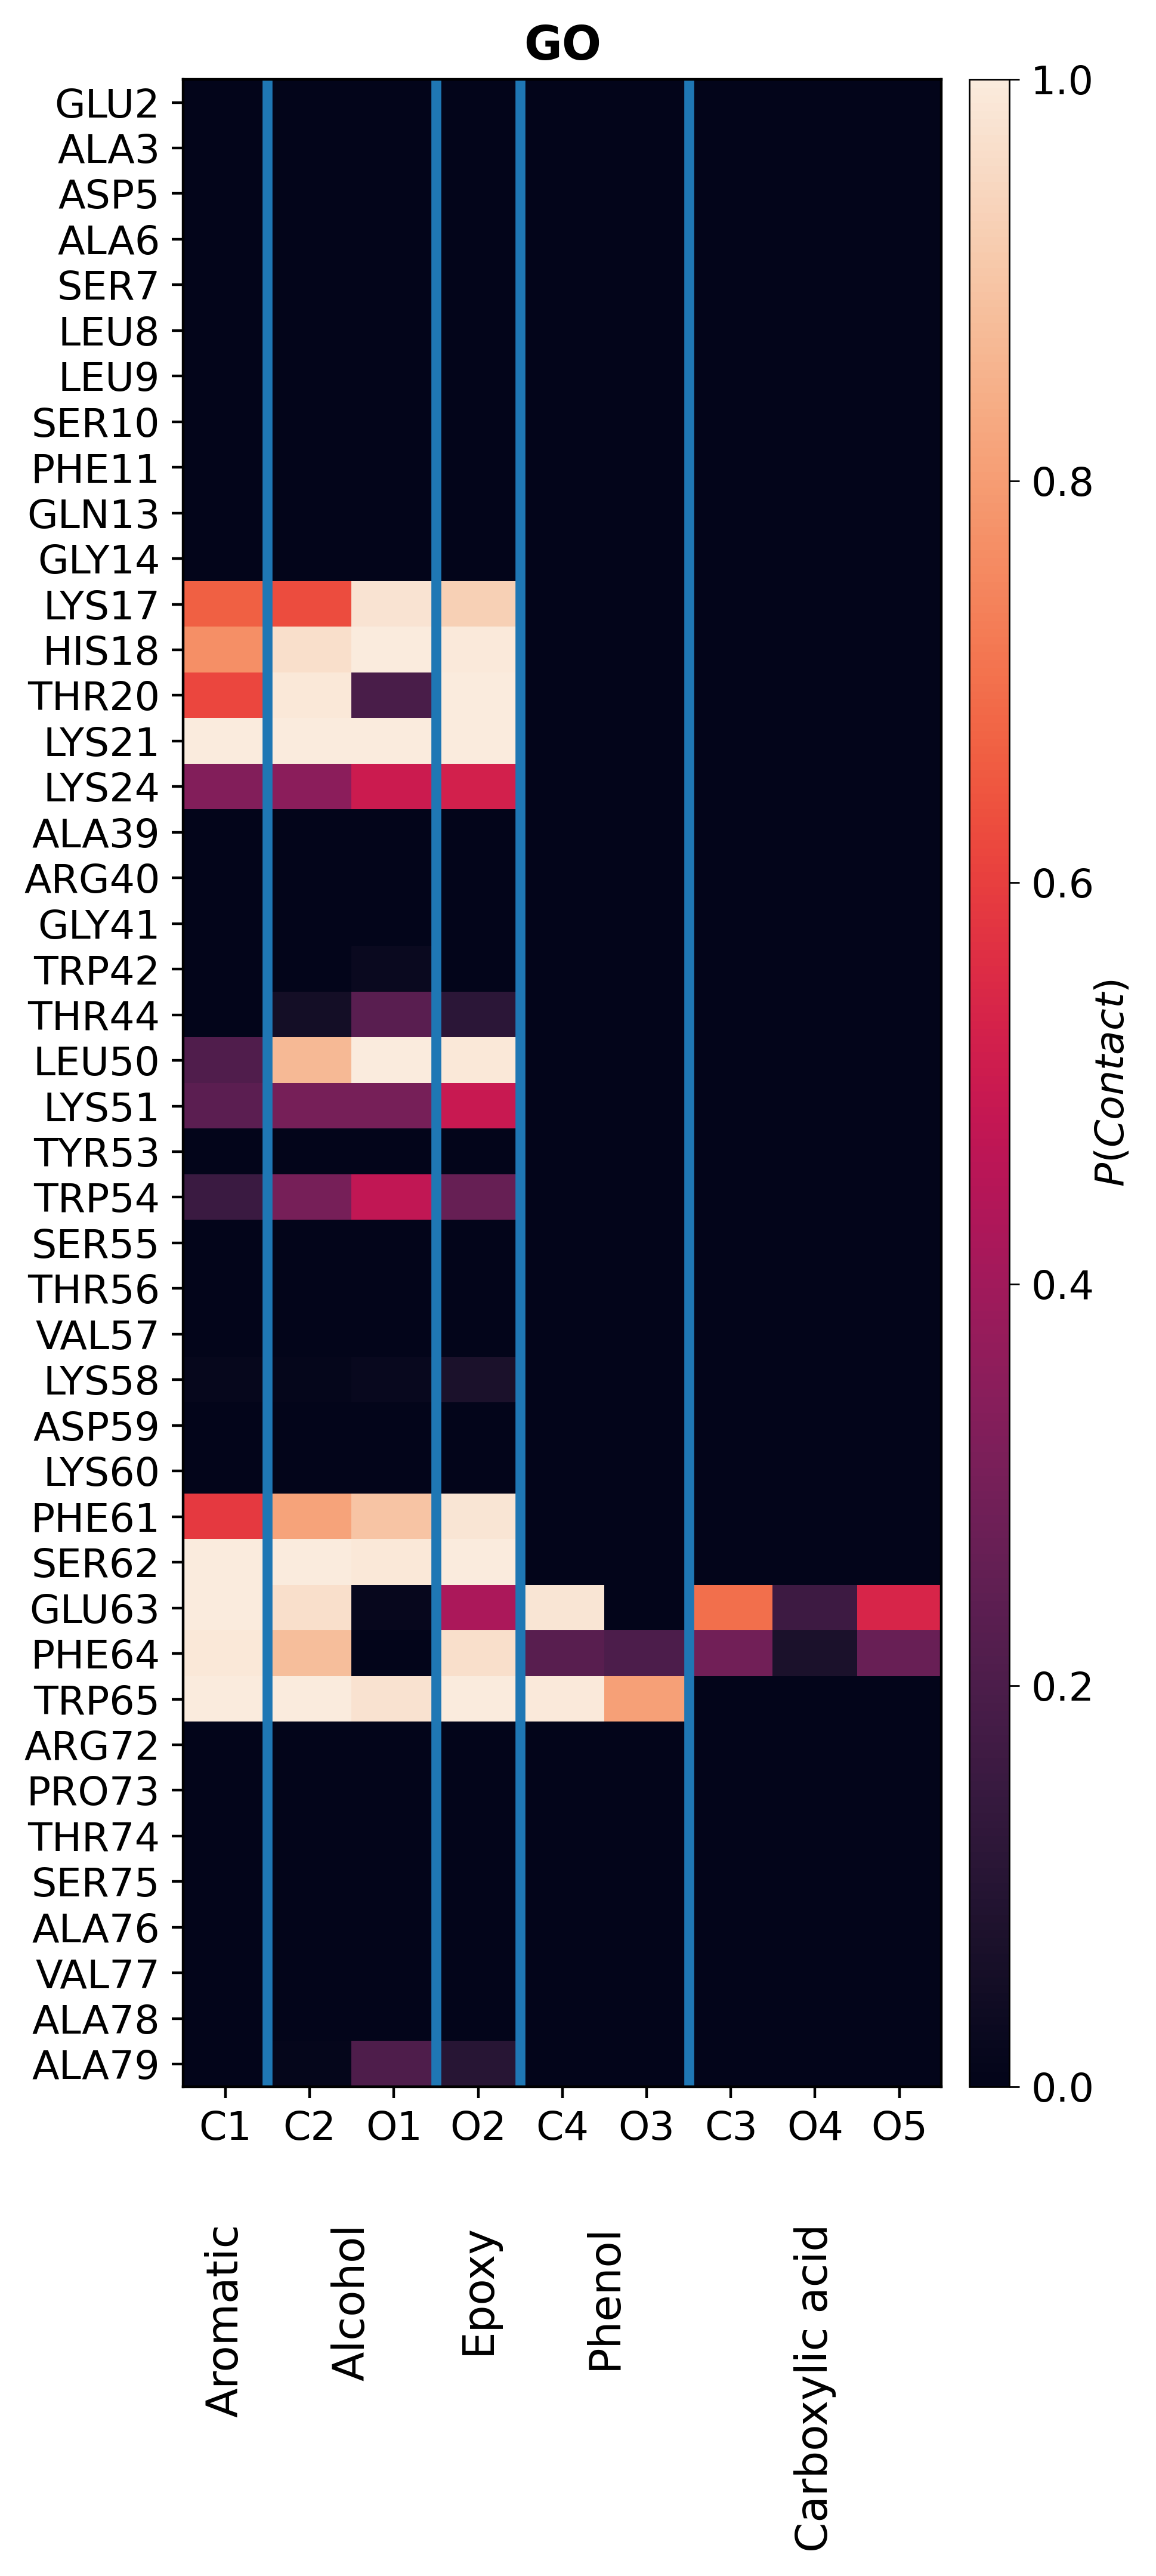
\includegraphics[height=18cm]{SI_go-OPLS-R1-residues-condensed_P01.png}
    \caption{Contact probability between each apo-C3 residue and each atom type of GO. Data from the final \SI{50}{\nano\second} of the trajectory. For clarity, only those residues with $P(\mathrm{Contact}) \geq 0.1$ for either GO or C2GO are shown.}
    \label{fig:prot-go-contacts}
\end{figure}

\begin{figure}
    \centering
    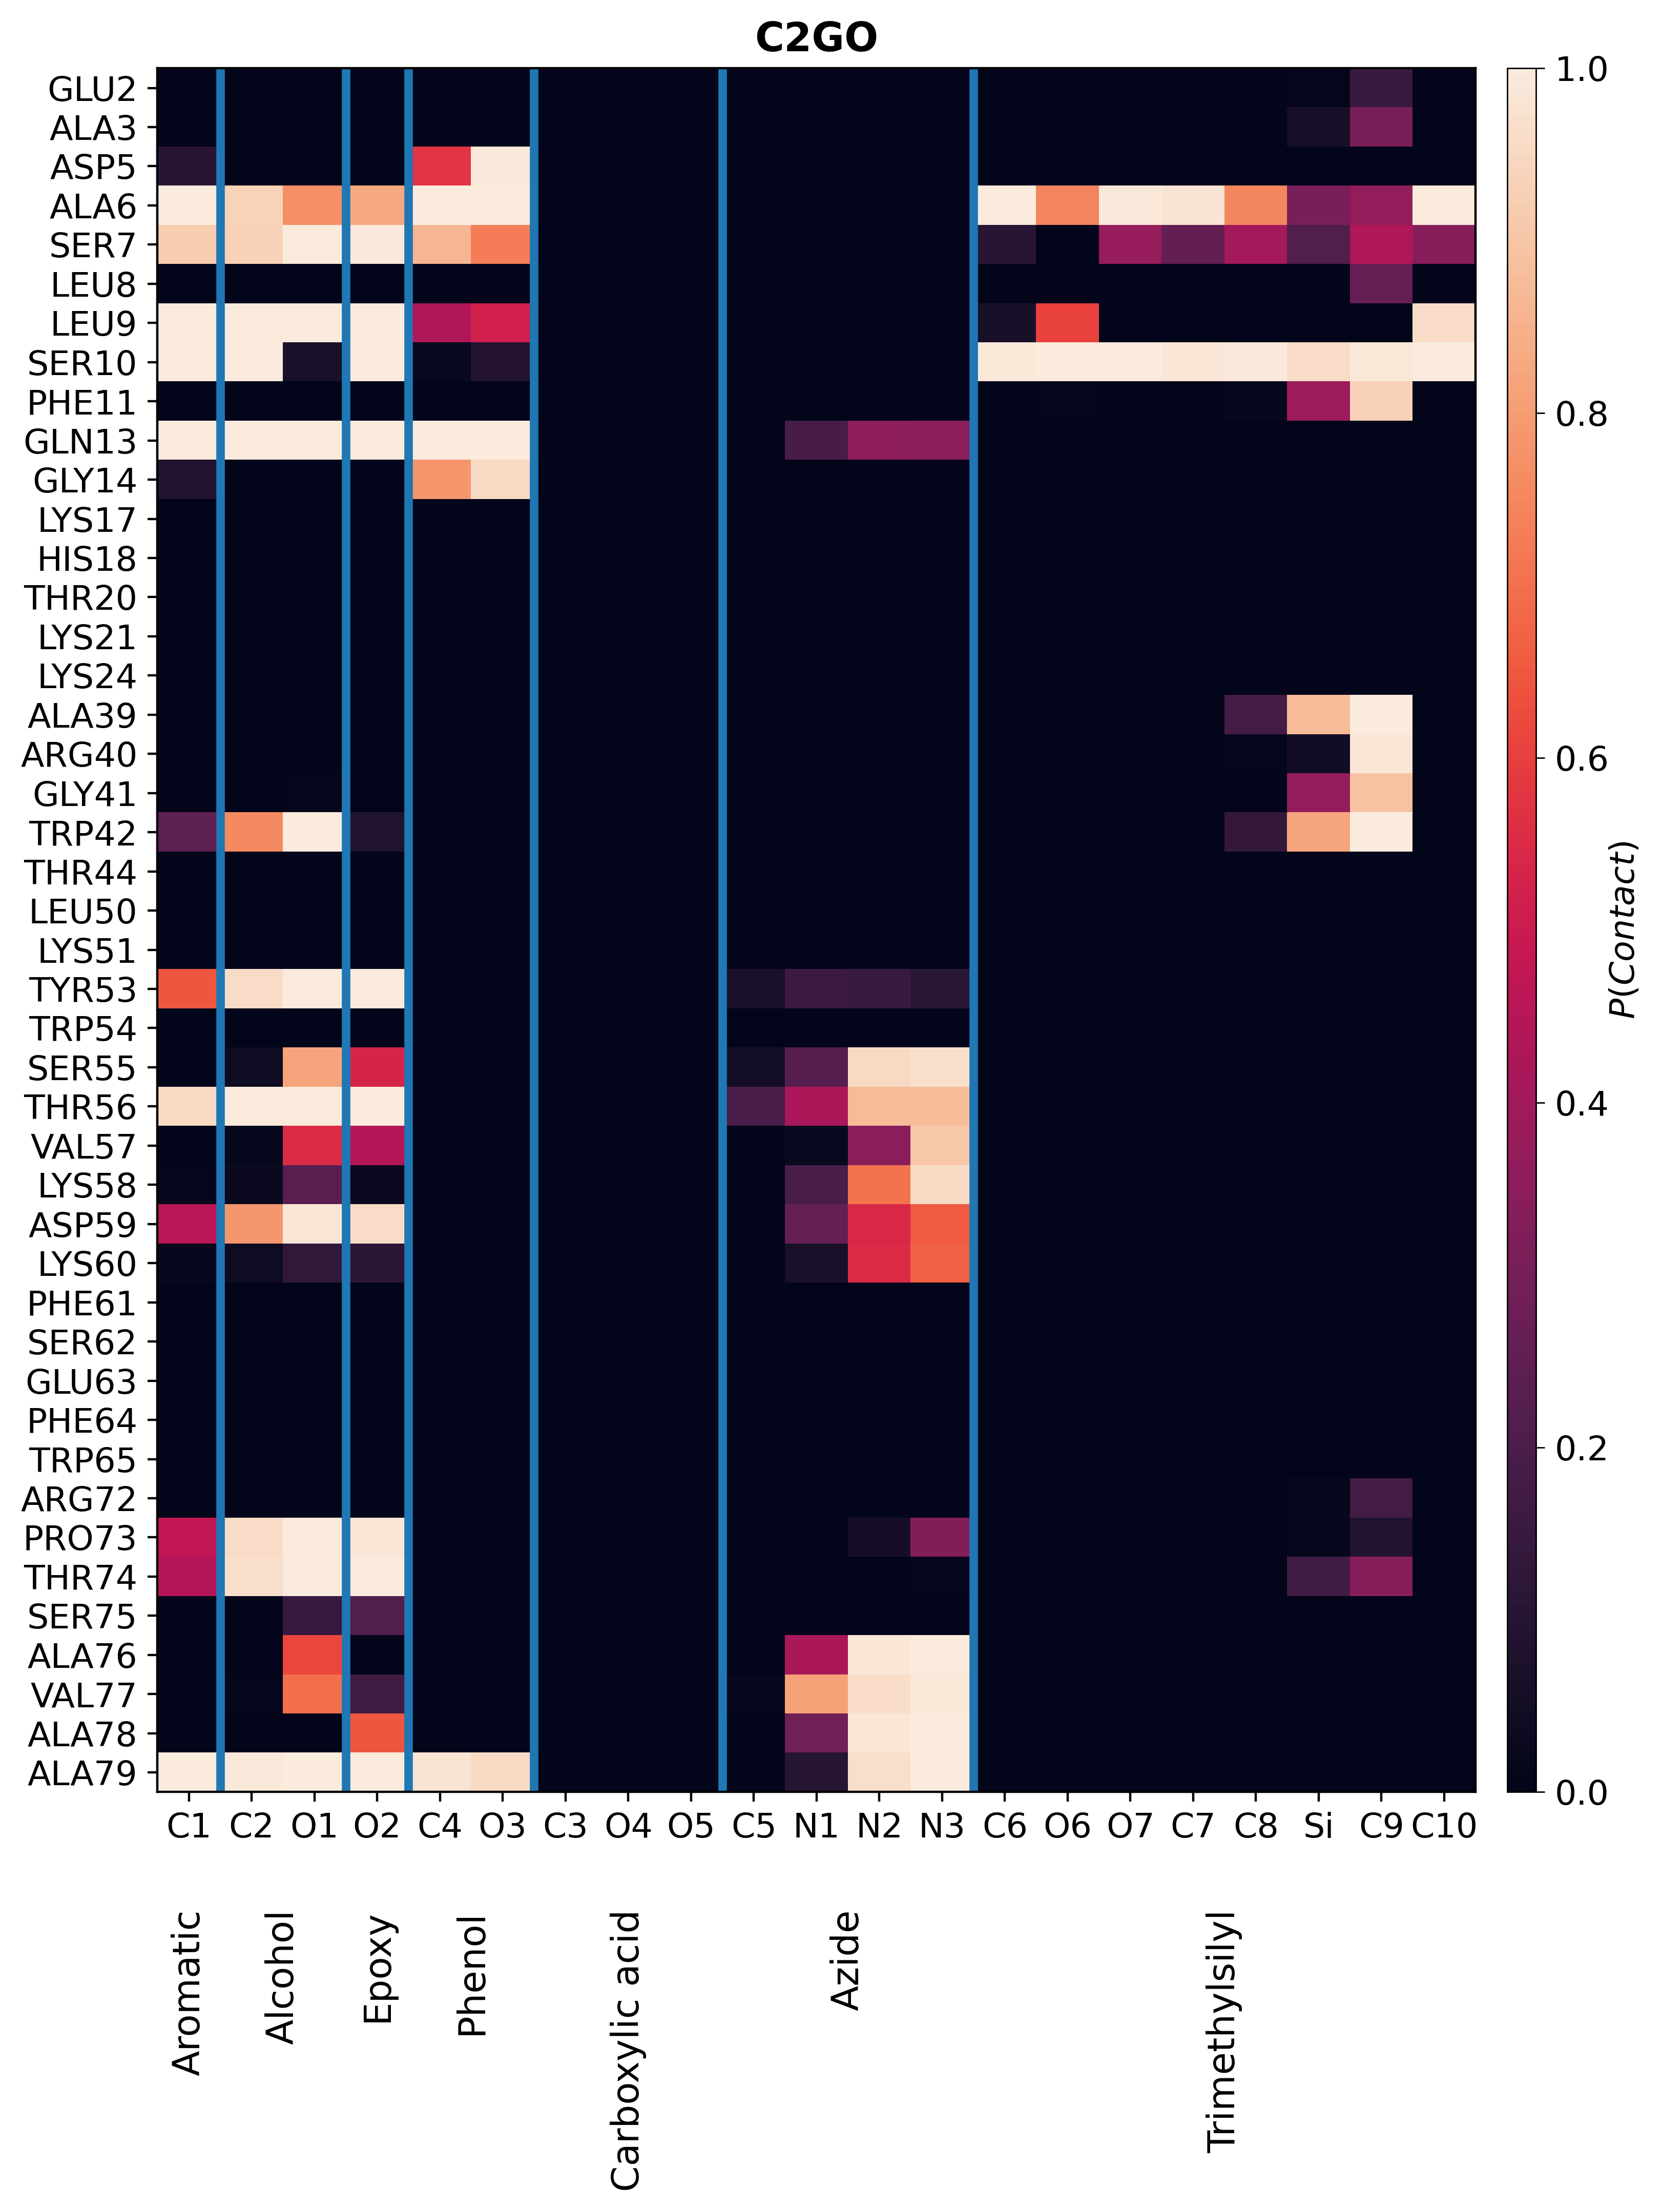
\includegraphics[height=18cm]{SI_c2go-OPLS-R2-residues-condensed_P01.png}
    \caption{Contact probability between each apo-C3 residue and each atom type of C2GO. Data from the final \SI{50}{\nano\second} of the trajectory. For clarity, only those residues with $P(\mathrm{Contact}) \geq 0.1$ for either GO or C2GO are shown.}
    \label{fig:prot-c2go-contacts}
\end{figure}
